\documentclass[aspectratio=169]{beamer}

% Theme and color scheme
\usetheme{Madrid}
\usecolortheme{seahorse}

% Packages
\usepackage[utf8]{inputenc}
\usepackage{graphicx}
\usepackage{amsmath}
\usepackage{amssymb}
\usepackage{tikz}
\usepackage{booktabs}
\usepackage{subcaption}
\usepackage{xcolor}

% Custom colors
\definecolor{rayblue}{RGB}{0, 122, 204}
\definecolor{awsorange}{RGB}{255, 153, 0}
\definecolor{hpcgreen}{RGB}{0, 153, 76}

% Title information
\title[Optimizing Vector Algorithm Processing]{Optimizing Vector Algorithm Processing through the integration of Ray IO and HPC in the Cloud}
\author{Tiago de Souza de Oliveira}
\institute[University]{
    Master's Thesis Defense \\
    Computer Science Department
}
\date{\today}

% Footer information
\setbeamertemplate{footline}[frame number]

\begin{document}

% Title slide
\frame{\titlepage}

% Index slide
\begin{frame}{Presentation Overview}
    \begin{columns}
        \begin{column}{0.48\textwidth}
            \textbf{\textcolor{rayblue}{Part I: Problem \& Architecture}}
            \begin{enumerate}
                \item \textbf{The New Frontier} \\
                \small Scientific workflow scaling \& HPC vs Cloud
                
                \item \textbf{Scientific Workflow Design} \\
                \small Data-centric pipeline \& token-to-embedding
                
                \item \textbf{Two-Phased Architecture} \\
                \small Separation of concerns \& metagenomics example
            \end{enumerate}
            
            \vspace{0.4cm}
            \textbf{\textcolor{hpcgreen}{Part II: Implementation}}
            \begin{enumerate}
                \setcounter{enumi}{3}
                \item \textbf{DNA Embedding Models} \\
                \small DNABERT-2, LSHVec, fastDNA \& Ray fitness
                
                \item \textbf{Phase 1: Ray ETL} \\
                \small Scalable preprocessing \& cost optimization
            \end{enumerate}
        \end{column}
        
        \begin{column}{0.48\textwidth}
            \begin{enumerate}
                \setcounter{enumi}{5}
                \item \textbf{Phase 2: HPC Simulation} \\
                \small ParallelCluster, GPU acceleration \& EFA
            \end{enumerate}
            
            \vspace{0.4cm}
            \textbf{\textcolor{awsorange}{Part III: Results \& Future}}
            \begin{enumerate}
                \setcounter{enumi}{6}
                \item \textbf{Conclusions} \\
                \small Key achievements \& scalability results
                
                \item \textbf{Future Directions} \\
                \small FPGA workloads \& Agentic AI for HPC
            \end{enumerate}
            
            \vspace{0.6cm}
            \begin{block}{Core Technical Contributions}
                \small
                \textbf{Architecture:} Cloud-native two-phase separation \\
                \textbf{Embeddings:} LSHVec optimization for metagenomics \\
                \textbf{Integration:} Ray + AWS ParallelCluster synergy \\
                \textbf{Storage:} S3 + FSx Lustre interoperability
            \end{block}
        \end{column}
    \end{columns}
\end{frame}

% Slide 1: The New Frontier
\begin{frame}{The New Frontier: Scaling Scientific Workflow with ETL and AI Workloads}
    \begin{columns}
        \begin{column}{0.8\textwidth}
            \textbf{Context \& Motivation:}
            \begin{itemize}
                \item \textbf{Scientific domains} (genomics, CFD) and \textbf{AI} (NLP, CV) demand processing of huge datasets.  
                \item Raw data is transformed into \textcolor{rayblue}{\textbf{dense embeddings}} for downstream algorithms.  
                \item \textbf{HPC pre-processing limits:} I/O bottlenecks, orchestration issues, and poor handling of unstructured data.  
                \item Map-Reduce/Spark \textbf{fall short at PB-scale and lack native support for AI model training}.  
            \end{itemize}
            
        \end{column}
        \begin{column}{0.2\textwidth}
            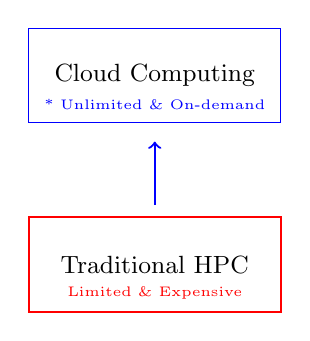
\begin{tikzpicture}[scale=0.8]
                % Traditional HPC box
                \draw[thick, red] (0,0) rectangle (4,1.5);
                \node at (2,0.75) {\small Traditional HPC};
                \node[red] at (2,0.3) {\tiny Limited \& Expensive};
                
                % Arrow
                \draw[->, thick, blue] (2, 1.7) -- (2, 2.7);
                
                % Cloud box
                \draw[blue] (0,3) rectangle (4,4.5);
                \node at (2,3.75) {\small Cloud Computing};
                \node[blue] at (2,3.3)  {\tiny * Unlimited \& On-demand};
            \end{tikzpicture}
        \end{column}
    \end{columns}
    
    \vspace{0.3cm}
        \begin{block}{The Opportunity}
        Cloud enables cost-efficient pipelines via IaC/DevOps, with \textbf{vectorizing as embeddings} (not HPC loop SIMD).  
        \end{block}
\end{frame}


% Slide 2: Scientific workflow
\begin{frame}{Scientific workflow}
    \begin{columns}
        \begin{column}{0.6\textwidth}
            \begin{itemize}
                \item \textbf{Data-centric pipeline}: raw inputs → structured embeddings → HPC simulations, with iterative feedback for performance and cost.  
                \item \textbf{Generative AI} enhances datasets and improves interoperability across processing engines.  
                \item \textbf{Embeddings} capture extra features and integrate seamlessly with numeric simulations.  
            \end{itemize}
        \end{column}
        \begin{column}{0.4\textwidth}
            \includegraphics[width=\textwidth,height=0.6\textheight,keepaspectratio]{../../images/DataCentric-DataBackbone-Strategy.png}
        \end{column}
    \end{columns}
    
    \vspace{0.3cm}
    \begin{block}{Key Insight}
        \textbf {Tokens become embeddings} through learned matrix multiplication plus positional encoding via vector addition
    \end{block}
\end{frame}

% Slide 3: A Two-Phased
\begin{frame}{A Two-Phased Cloud-Native Architecture for Optimization}
    % Upper row with bullet points
    \begin{itemize}
        \item \textbf{Scientific Workflow}: Requires high-throughput ETL, scalable HPC, distributed storage, and heterogeneous compute.
        \item \textbf{Separation of Concerns}: Ray handles data prep; Slurm/MPI handles simulations, ensuring modular scalability.
        \item \textbf{Metagenomic Read Clustering}: FASTQ reads → LSHVec embeddings → Parquet → HPC clustering.
        \item \textbf{Pipeline Value}: Efficient ETL–HPC handoff, enabling reproducibility, performance, and cost efficiency.
    \end{itemize}
        
    \vspace{0.3cm}
    \begin{block}{Workload Example}
        \textbf{Metagenomics}: FASTQ → k-mers → embeddings → organism clustering
    \end{block}
\end{frame}


% Slide 3: A Two-Phased
\begin{frame}{A Two-Phased Cloud-Native Architecture for Optimization}
    % Upper row with bullet points
        \vspace{0.4cm}
    
    % Bottom row with image
    \begin{center}
        \includegraphics[width=1\textwidth,height=0.6\textheight,keepaspectratio]{../../images/Generalized_data-pipeline.drawio.png}
    \end{center}
        
    \vspace{0.3cm}
    \begin{block}{Workload Example}
        \textbf{Metagenomics pipeline}  - FASTQ reads → k-mer embeddings → organism clustering
    \end{block}
\end{frame}


% Slide 4: Two-Phased Architecture
\begin{frame}{A Two-Phased Cloud-Native Architecture for Optimization}
    % Push diagram up a bit to leave room for footnotes
    \vspace{-0.8cm}
    \begin{center}
        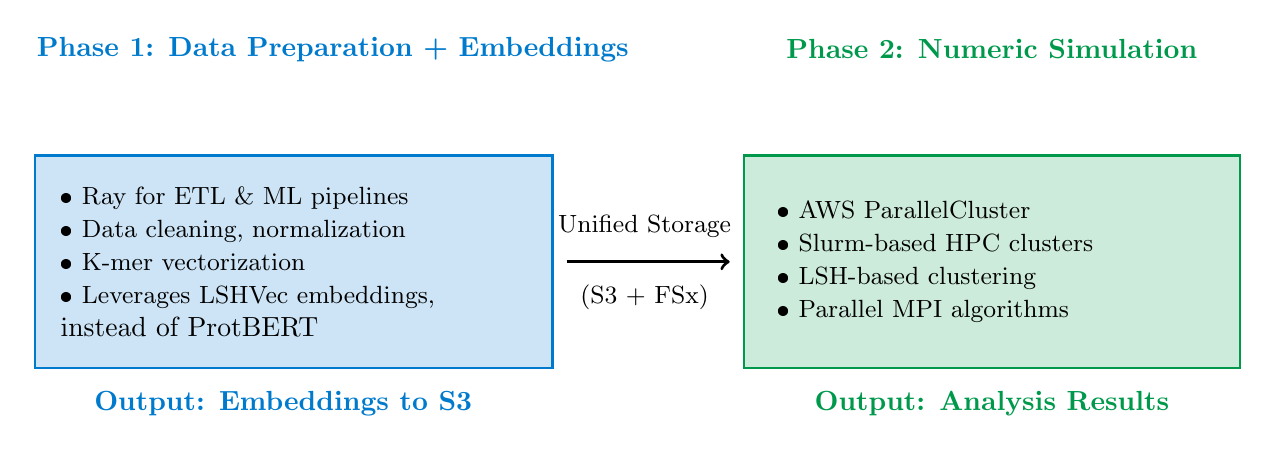
\begin{tikzpicture}[scale=0.9]
            % Phase 1 box
            \draw[thick, rayblue, fill=rayblue!20] (-3,0) rectangle (4.3,3);
            \node[rayblue, font=\bfseries] at (1.2,4.5) {Phase 1: Data Preparation + Embeddings};
            \node[align=left] at (0.0,1.5) {
                \small • Ray for ETL \& ML pipelines \\
                \small • Data cleaning, normalization \\
                \small • K-mer vectorization \\
                \small • Leverages LSHVec embeddings, \\ instead of ProtBERT
            };
            \node[rayblue] at (0.5,-0.5) {\textbf{Output: Embeddings to S3}};
            
            % Arrow
            \draw[->, very thick, black] (4.5, 1.5) -- (6.8, 1.5);
            \node at (5.6, 2) {\small Unified Storage};
            \node at (5.6, 1) {\small (S3 + FSx)};
            
            % Phase 2 box
            \draw[thick, hpcgreen, fill=hpcgreen!20] (7,0) rectangle (14,3);
            \node[hpcgreen, font=\bfseries] at (10.5,4.5) {Phase 2: Numeric Simulation};
            \node[align=left] at (9.7,1.5) {
                \small • AWS ParallelCluster \\
                \small • Slurm-based HPC clusters \\
                \small • LSH-based clustering \\
                \small • Parallel MPI algorithms
            };
            \node[hpcgreen] at (10.5,-0.5) {\textbf{Output: Analysis Results}};
        \end{tikzpicture}
    \end{center}
    
    % Reduce spacing after diagram to reclaim space
    \vspace{-0.4cm}
    \begin{block}{Key Integration}
        \textbf{Unified storage layer}: Seamless data flowing between stages and high-throughput access
        
        \textbf{To chain Phase 1 - Phase 2}: Event-driven workflow; Job Submit; pull-trigger-flag
    \end{block}
\end{frame}


% Slide 5: DNA Embedding Models for Ray Anyscale Deployment
\begin{frame}{DNA Embedding Models for Ray Anyscale Deployment}

\begin{itemize}
    \item \textbf{DNABERT-2:} SoTA accuracy, 322B+ DNA tokens, Ray HuggingFace integration
    \item \textbf{LSHVec:} Optimal scalability for terabyte-scale datasets with native distributed architecture and LSH optimization
    \item \textbf{fastDNA:} Fastest inference performance with lightweight k-mer embeddings
    \item \textbf{ProtBERT:} Protein-specific model incompatible with DNA sequences (amino acid vocabulary only)
\end{itemize}

\vfill

\begin{table}[b]
\centering
\tiny
\begin{tabular}{|p{2.2cm}|p{2.0cm}|p{2.0cm}|p{2.0cm}|p{2.0cm}|}
\hline
\textbf{Metric} & \textbf{DNABERT-2} & \textbf{LSHVec} & \textbf{fastDNA} & \textbf{ProtBERT} \\
\hline
\textbf{Primary Domain/ Training} & DNA (322B+ tokens) & DNA metagenomics & DNA metagenomics & Proteins (No DNA) \\
\hline
\textbf{Model Size} & 117M params & ~16M params & 10-100M params & 420M params \\
\hline
\textbf{Embedding Dimension} & 768 & 50-200 (config.) & 10-100 (config.) & 1024 \\
\hline
\textbf{Computation Optimization} & BPE + attention & LSH + skip-gram & k-mer embeddings & BERT masked LM \\
\hline
\textbf{Ray Fitness} & Excellent & Excellent & Good & Incompatible \\
\hline
\end{tabular}
\end{table}

    \vspace{0.3cm}
    \begin{block}{Tradeoff analysis}
        \textbf{Locality-Sensitive Hashing (LSH) Vec}: Designed for distributed training, to handle TB-scale datasets, hashing algorithm which dramatically reduces vocabulary size
    \end{block}

\end{frame}


% Slide 6: Phase 1
\begin{frame}{Phase 1 Deep Dive: Ray for Scalable Data Preprocessing}
    \begin{columns}
        \begin{column}{0.5\textwidth}
            \textbf{Ray's Role in Data Preparation:}
            \begin{itemize}
                \item \textbf{Data Ingestion:} Raw FASTQ reads processing as parquet files
                \item \textbf{K-mer Embeddings:} Using \textcolor{rayblue}{\textbf{LSHVec}} for fixed-length embeddings extraction
                \item \textbf{Parallel Processing:} Lightweight tasks across CPUs/GPUs
                \item \textbf{Output:} Parquet shards to Amazon S3 - FSxLustre
            \end{itemize}
        \end{column}
        \begin{column}{0.5\textwidth}
            \textbf{Performance \& Efficiency:}
            \begin{table}[h]
                \centering
                \small
                \begin{tabular}{lc}
                    \toprule
                    \textbf{Metric} & \textbf{Result} \\
                    \midrule
                    Scaling (1→2 GPUs) & (xx)× throughput \\
                    Processing rate & ~yy MB/s \\
                    Node startup time & ~xxs \\
                    Spot Instance savings & \textcolor{green}{\textbf{YY\%}} \\
                    Cost per GB & \textcolor{green}{\textbf{\$x.xx}} \\
                    \bottomrule
                \end{tabular}
            \end{table}
        \end{column}
    \end{columns}
    
    \vspace{0.3cm}
    \begin{block}{Key Achievement}
        \textbf{Fully automation} with Ray autoscaler dynamically managing cluster size and achieving operational and cost efficiency through Spot Instances
    \end{block}
\end{frame}

% Slide 7: Phase 2
\begin{frame}{Phase 2 Deep Dive: HPC ParallelCluster \& Overall Impact}

            \textbf{HPC Simulation with AWS ParallelCluster:}
            \begin{itemize}
                \item \textbf{Embedding Consumption:} Direct access from FSx/S3
                \item \textbf{Specialized Compute:} P4d instances with \textcolor{awsorange}{\textbf{NVIDIA A100 GPUs}}
                \item \textbf{Low-latency Communication:} Elastic Fabric Adapter (EFA) for MPI
                \item \textbf{Clustering Algorithms:} Parallel LSH and k-means for organism grouping
            \end{itemize}

    
    \vspace{0.3cm}
    \begin{block}{Synergistic Performance \& Benefits}
        \begin{itemize}
            
            \item \textbf{Extreme-scale Processing:} GPU acceleration for DNA sequencing processing
            \item \textbf{Developer Agility:} ParallelCluster automation for HPC cluster deployment
        \end{itemize}
    \end{block}
\end{frame}

% Slide 8: Conclusions
\begin{frame}{Conclusions}
    
            \textbf{Key Conclusions:}
            \begin{itemize}
                \item \textbf{Iterative feedback loop} 
                \item Cloud Two-phase architecture delivers \textbf{significant gains} in elasticity, performance, interoperability and cost-efficiency
                \item Automated life-cycle management and Spot Instances ensure {\textbf{optimized resource utilization}}
                \item Successfully \textbf{decouples feature engineering from raw simulation workloads}
                
            \end{itemize}
        
    
    \vspace{0.3cm}
    \begin{block}{Key achievements}
        \begin{itemize}
            \item \textbf{Ray autoscaler (EC2 + GPU):} Maximize scalability for \textbf{DNA embedding extraction}
            \item \textbf{Storage at scale S3 FsxLustre:} Ease data interoperability
        \end{itemize}
    \end{block}
\end{frame}

% Slide 9: Future Directions
\begin{frame}{Future Directions}


    \textbf{Key Emerging Capabilities:}
    \begin{itemize}
        \item \textcolor{rayblue}{\textbf{GPU-accelerated Ray clusters}} for scalable DNA embeddings
        \item Serverless ETL (AWS Glue) vs. Ray for preprocessing efficiency
        \item \textbf{Elastic Fabric Adapter + FSx Lustre} for low-latency, high-throughput HPC I/O
    \end{itemize}

    \vspace{0.3cm}
    \begin{block}{Future Work \& Research}
        \begin{itemize}
            \item \textbf{FPGA acceleration} (AWS F1) for Smith-Waterman alignment
            \item \textbf{Apple M-Series} exploration via Metal for scientific inference
            \item \textbf{Agentic AI in HPC:} workflow/simulation agents with iterative feedback
            \item Continue investigations to validate and refine initial hypotheses
        \end{itemize}
    \end{block}
\end{frame}


% Thank you slide
\begin{frame}[plain]
    \begin{center}
        \Huge Thank You!
        
        \vspace{1cm}
        \Large Questions?
        
        \vspace{0.8cm}
        \normalsize
        \textbf{Optimizing Vector Algorithm Processing through the integration of Ray IO and HPC in the Cloud}
        
        \vspace{0.5cm}
        Tiago de Souza de Oliveira \\
        \texttt{tiago.souza@rai.usc.es, tiagoooliveira@qmind-lab.com}
    \end{center}
\end{frame}

\end{document}